\section{極限}\label{chap-8-limit}

\begin{define}[極限]\label{def-limit}
  ある圏$\cat{C},\cat{D}$と関手$\functor{F}{C}{D}$に対する極限$(\lim F, \nu)$を以下のように構成する。
  \begin{quote}
    \begin{mydescription}
      \item[錐] 錐と呼ばれる組$(X,\mu)$を以下のように構成する。
      圏$\cat{D}$の対象である$X$と、
      圏$\cat{C}$の任意の対象$C$に対して$\mor{\mu_C}{X}{FC}$なる射が存在し、圏$\cat{C}$の任意の射$\mor{f}{A}{B}$に対して$\mu_B=Ff\circ\mu_A$が成り立つ。
      \begin{center}
        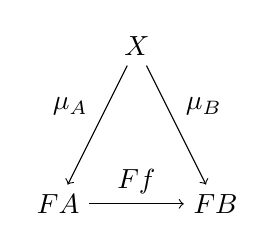
\begin{tikzpicture}[auto]
          \node (limf) at (0, 2) {$X$};
          \node (fa) at (-1, 0) {$FA$};
          \node (fb) at (1, 0) {$FB$};
          \draw[->] (limf) to node[swap]{$\mu_A$}(fa);
          \draw[->] (limf) to node{$\mu_B$}(fb);
          \draw[->] (fa) to node{$Ff$}(fb);
        \end{tikzpicture}
      \end{center}
      
      またこの対象ごとの射は自然変換で表せる。$\mor{\mu}{\Delta X}{F}$とすると、対象$C$の成分は$\mor{\mu_C}{X}{FC}$であり、等式$\mu_B=Ff\circ\mu_A$は自然変換の自然性にあたる。
      \begin{center}
        \begin{tikzpicture}[auto]
          \node (catc) at (-4, 3) {$\cat{C}$};
          \node (a) at (-5, 1) {$A$};
          \node (b) at (-3, 1) {$B$};
          \draw[->] (a) to node{$f$}(b);

          \node (catd) at (0, 3) {$\cat{D}$};
          \node (limf) at (0, 2) {$X$};
          \node (fa) at (-1, 0) {$FA$};
          \node (fb) at (1, 0) {$FB$};
          \draw[->] (limf) to node[swap]{$\mu_A$}(fa);
          \draw[->] (limf) to node{$\mu_B$}(fb);
          \draw[->] (fa) to node{$Ff$}(fb);

          \draw[->,bend left = 20] (catc) to node (funcf){$\varDelta X$}(catd);
          \draw[->,bend right = 20] (catc) to node (funcg)[swap]{$F$}(catd);
          \draw[double,double equal sign distance,-implies,shorten >=5pt,shorten <=5pt] (funcf) -- node[label=right:$\mu$] {} (funcg);
        \end{tikzpicture}
      \end{center}
      \item[普遍性] ある錐$(\lim F, \tau)$が極限であるとは、他の錐$(X,\mu)$に対して、$\tau_C = \nu_C\circ h$が成り立つような$\mor{h}{X}{\lim F}$が一意に存在する。すなわち自然変換$\mu$は$\tau$によって単なる射$h$へと分解される。
      また、この時一意に定まる射を$\mor{\tuple{\mu}}{X}{\lim F}$と表記することにする。
      \begin{center}
        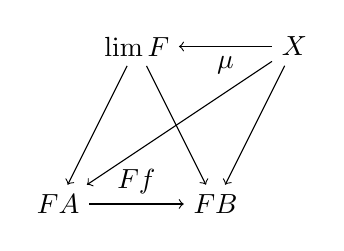
\begin{tikzpicture}[auto]
          \node (limf) at (0, 2) {$\lim F$};
          \node (x) at (2, 2) {$X$};

          \node (fa) at (-1, 0) {$FA$};
          \node (fb) at (1, 0) {$FB$};
          \draw[->] (limf) to node{}(fa);
          \draw[->] (limf) to node{}(fb);
          \draw[->] (x) to node[swap]{}(fa);
          \draw[->] (x) to node{}(fb);
          \draw[->] (fa) to node{$Ff$}(fb);
          \draw[->] (x) to node{$\tuple{\mu}$}(limf);
        \end{tikzpicture}
        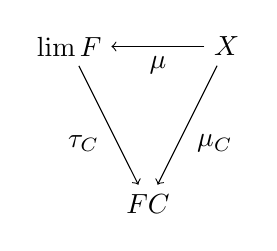
\begin{tikzpicture}[auto]
          \node (limf) at (0, 2) {$\lim F$};
          \node (x) at (2, 2) {$X$};

          \node (fa) at (1, 0) {$FC$};
          \draw[->] (limf) to node[swap]{$\tau_C$}(fa);
          \draw[->] (x) to node{$\mu_C$}(fa);
          \draw[->] (x) to node{$\tuple{\mu}$}(limf);
        \end{tikzpicture}
      \end{center}
      この時、$\lim F$を極限対象や極限、$\tau_C$を極限における射影射と呼ぶことにする。
    \end{mydescription}
  \end{quote}
\end{define}

\begin{prop}[極限の分配則]
  極限$(\lim F, \tau)$と錐$(X ,\mu)$、射$\mor{h}{Y}{X}$に対して
  \[\tuple{\mu}\circ h = \tuple{\mu\circ\varDelta h}\]
\end{prop}
\begin{proof}
  定自然変換の定義より、任意の対象$C$に対して$(\varDelta h)_C=h$である。よって自然変換の垂直合成より\[\mu_C\circ h = \mu_C\circ (\varDelta h)_C = (\mu\cdot \varDelta h)_C\]よって$ \mu_C\circ h$は自然変換となるから、$\mor{\tuple{\mu\cdot\varDelta h}}{Y}{\lim F}$なる射が一意に存在する。すると$\tuple{\mu}\circ h$もまた\[\tau_C\circ(\tuple{\mu}\circ h)=\mu_C\circ h\]を満たす。よって射の一意性より、$\tuple{\mu}\circ h = \tuple{\mu\circ\varDelta h}$となる。
  \begin{center}
    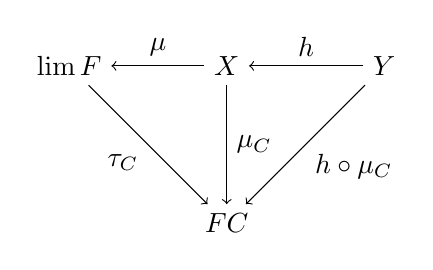
\begin{tikzpicture}[auto]
      \node (limf) at (0, 2) {$\lim F$};
      \node (x) at (2, 2) {$X$};
      \node (limf2) at (4, 2) {$Y$};
      \node (fa) at (2, 0) {$FC$};
      \draw[->] (limf) to node[swap]{$\tau_C$}(fa);
      \draw[->] (x) to node{$\mu_C$}(fa);
      \draw[->] (limf2) to node{$h\circ\mu_C$}(fa);
      \draw[->] (x) to node[swap]{$\tuple{\mu}$}(limf);
      \draw[->] (limf2) to node[swap]{$h$}(x);
    \end{tikzpicture}
    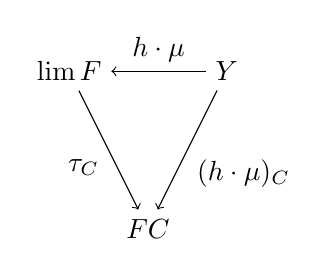
\begin{tikzpicture}[auto]
      \node (limf) at (0, 2) {$\lim F$};
      \node (x) at (2, 2) {$Y$};

      \node (fa) at (1, 0) {$FC$};
      \draw[->] (limf) to node[swap]{$\tau_C$}(fa);
      \draw[->] (x) to node{$(\varDelta h\cdot \mu)_C$}(fa);
      \draw[->] (x) to node[swap]{$\tuple{\varDelta h\cdot \mu}$}(limf);
    \end{tikzpicture}
  \end{center}
\end{proof}
\begin{prop}[極限の一意性]\label{prop-uniqueness-of-limits}
  関手$F$に対する極限$(\lim F, \tau)$が存在するとする。同様に$(X, \mu)$も関手$F$に対する極限であるならば、$\lim F\cong X$である。
\end{prop}
\begin{proof}
  積や終対象の一意性と同様に証明する。

  極限の定義から、$\mor{\tuple{\mu}}{X}{\lim F}$なる射が一意に存在するが、同時に$X$も極限対象であるから$\mor{\tuple{\tau}}{\lim F}{X}$が一意に存在する。この二つの射が同型射になることを示せば良い。

  以下の図式から、$\tau_C =\tau_C\circ \tuple{\tau}\circ \tuple{\mu}$となる$\tuple{\tau}\circ \tuple{\mu}$は極限の普遍性によって一意に定まるが、同様に恒等射$\mor{id_{lim F}}{lim F}{lim F}$も$\tau_C =\tau_C \circ id_{lim F}$であるから、一意性より$\tuple{\tau}\circ \tuple{\mu}=id_{lim F}$となる。

  同様に$\tuple{\mu}\circ \tuple{\tau} = id_X$も示せるから$\lim F\cong X$である。

  \begin{center}
    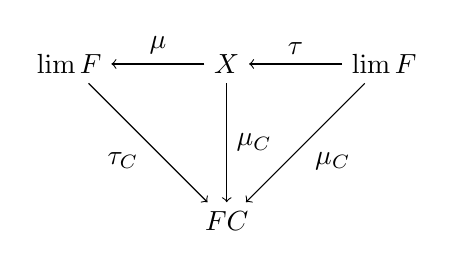
\begin{tikzpicture}[auto]
      \node (limf) at (0, 2) {$\lim F$};
      \node (x) at (2, 2) {$X$};
      \node (limf2) at (4, 2) {$\lim F$};
      \node (fa) at (2, 0) {$FC$};
      \draw[->] (limf) to node[swap]{$\tau_C$}(fa);
      \draw[->] (x) to node{$\mu_C$}(fa);
      \draw[->] (limf2) to node{$\mu_C$}(fa);
      \draw[->] (x) to node[swap]{$\tuple{\mu}$}(limf);
      \draw[->] (limf2) to node[swap]{$\tuple{\tau}$}(x);
    \end{tikzpicture}
    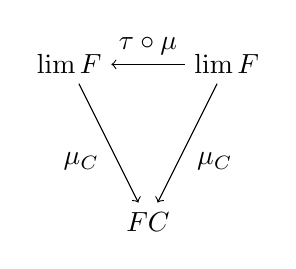
\begin{tikzpicture}[auto]
      \node (limf) at (0, 2) {$\lim F$};
      \node (x) at (2, 2) {$\lim F$};

      \node (fa) at (1, 0) {$FC$};
      \draw[->] (limf) to node[swap]{$\mu_C$}(fa);
      \draw[->] (x) to node{$\mu_C$}(fa);
      \draw[->] (x) to node[swap]{$\tuple{\tau}\circ \tuple{\mu}$}(limf);
    \end{tikzpicture}
  \end{center}
\end{proof}
\begin{define}[完備]\label{def-completeness}
  圏$\cat{D}$が完備であるとは、任意の関手$\functor{F}{C}{D}$に対して極限$(\lim F, \tau)$を持つことである。
\end{define}
% \begin{prop}[集合の圏の完備性]
%   集合の圏$\cat{Set}$は完備である。
% \end{prop}
% \begin{proof}
%   任意の関手$\functor{F}{C}{Set}$と、終対象$1$への定関手$\functor{\varDelta 1}{C}{Set}$の間の自然変換の集合$\arset{\funccat{C}{D}}{\varDelta 1}{F}$を考える。これをエンドと見なしたときの
% \end{proof}
\begin{prop}\label{prop-def-limit-by-arrowset}
  任意の対象$X$、任意の関手$\functor{F}{C}{D}$において\[\arset{D}{X}{\lim F}\cong\arset{\funccat{C}{D}}{\varDelta X}{F}\]
\end{prop}
\begin{proof}
  自然変換の集合はエンドで表せたから、エンドの一意性を用いて証明する。すなわち$\arset{D}{X}{\lim F}$が$\functor{\arset{D}{\varDelta X (-)}{F-}}{C}{Set}$におけるエンドであることを示せばよい。
  \begin{center}
    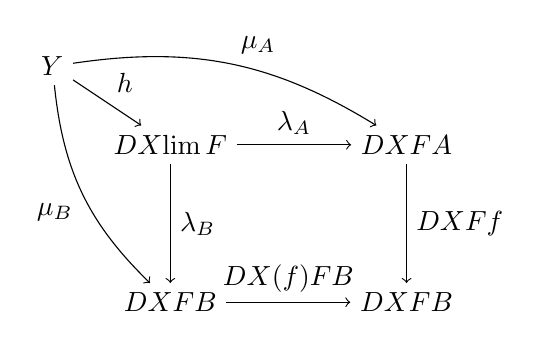
\begin{tikzpicture}[auto]
      \node (X) at (-1.5, 1) {$Y$};

      \node (FG) at (0, 0) {$\arset{D}{X}{\lim F}$};
      \node (FAGA) at (3, 0) {$\arset{D}{X}{FA}$};
      \node (FBGB) at (0, -2) {$\arset{D}{X}{FB}$};
      \node (FAGB) at (3, -2) {$\arset{D}{X}{FB}$};
      \draw[->] (X) to node{$h$}(FG);

      \draw[->,bend left = 20] (X) to node{$\mu_A$}(FAGA);
      \draw[->,bend right = 20] (X) to node[swap]{$\mu_B$}(FBGB);
      \draw[->] (FG) to node{$\lambda_A$}(FAGA);
      \draw[->] (FG) to node{$\lambda_B$}(FBGB);
      \draw[->] (FAGA) to node{$\arset{D}{X}{Ff}$}(FAGB);
      \draw[->] (FBGB) to node{$\arset{D}{\varDelta X(f)}{FB}$}(FAGB);
    \end{tikzpicture}
  \end{center}
  ただしエンドの図式における$\arset{D}{\varDelta X(f)}{FB}$は$\varDelta X(f)=id_X$により$id_{\arset{D}{X}{FB}}$である。
  
  すると少しわかりにくいが、$\lambda_C=\tau_C$とすると前の共変Hom関手の極限の保存の図式そのものとなる。よって$\arset{D}{X}{\lim F}$の極限の普遍性によって$\arset{D}{X}{\lim F}$のエンドの普遍性を満たす。よって$(\arset{D}{X}{\lim F}, \tau)$は極限でもあり、ある種のエンドになることが分かった。ゆえにエンドの一意性から\[\arset{D}{X}{\lim F}\cong\arset{\funccat{C}{D}}{\varDelta X}{F}\]が成り立つ。
\end{proof}
またエンドと極限の関係として以下の命題が成り立つ。
\begin{prop}[エンドによる極限の定義]
  任意の関手$\functor{F}{C}{D}$に対して$T(A,B)=F(B)$となるような関手$\functor{T}{C^{op}\times C}{D}$を考える。この時、
  関手$T$に対するエンド$(\cend{C}{C}T(C,C),\lambda)$は$F$に対する極限となる。
\end{prop}
\begin{proof}
  エンド$(\cend{C}{C}T(C,C),\lambda)$は、任意の射$\mor{f}{B}{A}$に対して
  \[T(A,f)\circ\lambda_A=T(f,B)\circ\lambda_B\]が成り立ち、かつ
  \[T(A,f)\circ\mu_A=T(f,B)\circ\mu_B\]となるような$\mor{\mu_C}{X}{T(C,C)}$が存在するとき、$\mu_C = \lambda_C\circ h$が成り立つような$\mor{h}{X}{\cend{C}{C}T(C,C)}$が一意に存在する。という普遍性を持つのであった。
  \begin{center}
    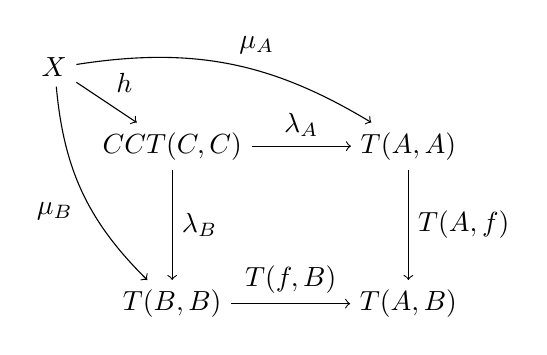
\begin{tikzpicture}[auto]
      \node (FG) at (0, 0) {$\cend{C}{C} T(C,C)$};
      \node (X) at (-1.5, 1) {$X$};
      \node (FAGA) at (3, 0) {$T(A,A)$};
      \node (FBGB) at (0, -2) {$T(B,B)$};
      \node (FAGB) at (3, -2) {$T(A,B)$};

      \draw[->] (FG) to node{$\lambda_A$}(FAGA);
      \draw[->] (X) to node{$h$}(FG);

      \draw[->] (FG) to node{$\lambda_B$}(FBGB);
      \draw[->,bend left = 20] (X) to node{$\mu_A$}(FAGA);
      \draw[->,bend right = 20] (X) to node[swap]{$\mu_B$}(FBGB);
      \draw[->] (FAGA) to node{$T(A,f)$}(FAGB);
      \draw[->] (FBGB) to node{$T(f,B)$}(FAGB);
    \end{tikzpicture}
  \end{center}
  ここで$T(A,B)=F(B)$を用いると、\[T(A,B)=F(B)=T(B,B),\ F(f,B)=id_{FB}\]が成り立つ。よってエンドの普遍性は以下のように置き換えられる。

  任意の射$\mor{f}{B}{A}$に対して
  \[F(f)\circ\lambda_A=\lambda_B\]が成り立ち、かつ
  \[F(f)\circ\mu_A=\mu_B\]となるような$\mor{\mu_C}{X}{F(C)}$が存在するとき、$\mu_C = \lambda_C\circ h$が成り立つような$\mor{h}{X}{\cend{C}{C}F(C)}$が一意に存在する。
  \begin{center}
    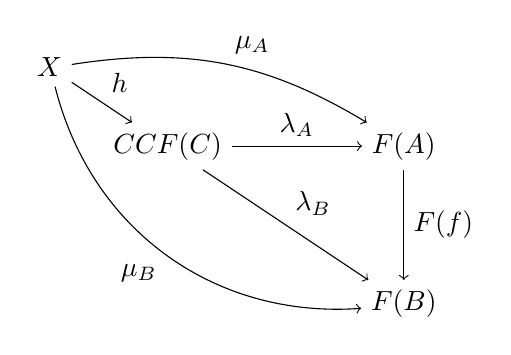
\begin{tikzpicture}[auto]
      \node (FG) at (0, 0) {$\cend{C}{C} F(C)$};
      \node (X) at (-1.5, 1) {$X$};
      \node (FAGA) at (3, 0) {$F(A)$};
      \node (FAGB) at (3, -2) {$F(B)$};

      \draw[->] (FG) to node{$\lambda_A$}(FAGA);
      \draw[->] (X) to node{$h$}(FG);

      \draw[->] (FG) to node{$\lambda_B$}(FAGB);
      \draw[->,bend left = 20] (X) to node{$\mu_A$}(FAGA);
      \draw[->,bend right = 40] (X) to node[swap]{$\mu_B$}(FAGB);
      \draw[->] (FAGA) to node{$F(f)$}(FAGB);
    \end{tikzpicture}
  \end{center}
  このように極限の定義と完全に一致する。よって$(\cend{C}{C}F(C),\lambda)$は関手$F$に対する極限である。
\end{proof}
\begin{prop}[同型の極限の保存]
  関手$\functor{F}{C}{D}$に対して$\lim F$が$F$に対する極限対象であり、$\lim F\cong X$であるならば、$X$もまた極限対象である。
\end{prop}
\begin{proof}
  同型のエンドの保存より明らかに成り立つ。
\end{proof}
\begin{prop}[極限の関手性]\label{prop-limit-is-functor}
  圏$\cat{D}$が完備であるとする。任意の関手$\functor{F}{C}{D}$に対して極限対象$\lim F$を得る操作は関手である。すなわち$\mor{\lim}{\funccat{C}{D}}{D}$である。
\end{prop}
\begin{proof}
  \begin{quote}~
    \begin{mydescription}
      \item[対象関数] 任意の関手$\functor{F}{C}{D}$に対して対象関数を$\lim(F) = \lim F$と定義する。
      \item[射関数] 
      任意の自然変換$\nat{\alpha}{F}{G}$に対して、射関数によって写された射$\lim \alpha$を考える。

      関手$F,G$による極限を$(\lim F, \tau),(\lim G, \nu)$とすると、極限$(\lim G, \nu)$の普遍性より$\mor{\tuple{\alpha\cdot\tau}}{\lim F}{\lim G}$への射が一意に存在する。
      \begin{center}
        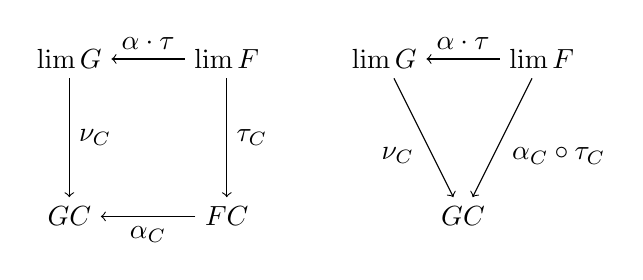
\begin{tikzpicture}[auto]
          \node (limf) at (2, 0) {$\lim F$};
          \node (limg) at (0, 0) {$\lim G$};

          \node (fa) at (2, -2) {$FC$};
          \node (ga) at (0, -2) {$GC$};
          \draw[->] (limf) to node{$\tau_C$}(fa);
          \draw[->] (limg) to node{$\nu_C$}(ga);
          \draw[->] (fa) to node{$\alpha_C$}(ga);
          \draw[->] (limf) to node[swap]{$\tuple{\alpha\cdot\tau}$}(limg);

          \node (limf) at (4, 0) {$\lim G$};
          \node (x) at (6, 0) {$\lim F$};
    
          \node (fa) at (5, -2) {$GC$};
          \draw[->] (limf) to node[swap]{$\nu_C$}(fa);
          \draw[->] (x) to node{$\alpha_C\circ \tau_C$}(fa);
          \draw[->] (x) to node[swap]{$\tuple{\alpha\cdot\tau}$}(limf);
        \end{tikzpicture}
      \end{center}
      この射を$\lim\alpha$とする。すなわち$\lim(\alpha)=\tuple{\alpha\cdot\tau}$である。
      \item[恒等射の保存] $\lim(ID_F)=id_{\lim F}$を示せば良い。$\tau_C\circ id_{\lim F} = \tau_C$であるが、極限の普遍性よりこのような射は一意に定まる。よって$\tuple{\tau}=id_{\lim F}$であり恒等射を保つ。
      \begin{center}
        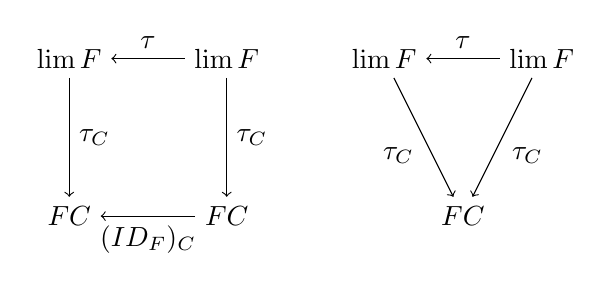
\begin{tikzpicture}[auto]
          \node (limf) at (2, 0) {$\lim F$};
          \node (limg) at (0, 0) {$\lim F$};

          \node (fa) at (2, -2) {$FC$};
          \node (ga) at (0, -2) {$FC$};
          \draw[->] (limf) to node{$\tau_C$}(fa);
          \draw[->] (limg) to node{$\tau_C$}(ga);
          \draw[->] (fa) to node{$(ID_F)_C$}(ga);
          \draw[->] (limf) to node[swap]{$\tuple{\tau}$}(limg);

          \node (limf) at (4, 0) {$\lim F$};
          \node (x) at (6, 0) {$\lim F$};
    
          \node (fa) at (5, -2) {$FC$};
          \draw[->] (limf) to node[swap]{$\tau_C$}(fa);
          \draw[->] (x) to node{$\tau_C$}(fa);
          \draw[->] (x) to node[swap]{$\tuple{\tau}$}(limf);
        \end{tikzpicture}
      \end{center}
      \item[射の合成の保存] $\lim (\beta\cdot\alpha)=\lim \beta\circ \lim\alpha$を示せば良い。極限$(\lim F,\tau),(\lim G,\nu),(\lim H,\mu)$と自然変換$\nat{\alpha}{F}{G},\ \nat{\beta}{G}{H}$に対して、
      \[(\beta\cdot\alpha)_C\circ\tau_C=\mu_C\circ\lim\beta\circ\lim\alpha \]が成り立つが、射関数の定義と射の一意性により$\lim (\beta\cdot\alpha)=\lim\beta\circ\lim\alpha$が成り立つ。
      \begin{center}
        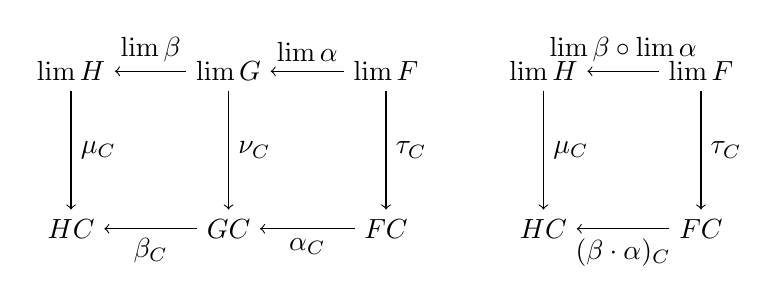
\begin{tikzpicture}[auto]
          \node (limf) at (2, 0) {$\lim F$};
          \node (limg) at (0, 0) {$\lim G$};
          \node (limh) at (-2, 0) {$\lim H$};

          \node (fa) at (2, -2) {$FC$};
          \node (ga) at (0, -2) {$GC$};
          \node (ha) at (-2, -2) {$HC$};

          \draw[->] (limf) to node{$\tau_C$}(fa);
          \draw[->] (limg) to node{$\nu_C$}(ga);
          \draw[->] (limh) to node{$\mu_C$}(ha);

          \draw[->] (fa) to node{$\alpha_C$}(ga);
          \draw[->] (ga) to node{$\beta_C$}(ha);

          \draw[->] (limf) to node[swap]{$\lim \alpha$}(limg);
          \draw[->] (limg) to node[swap]{$\lim \beta$}(limh);


          \node (limf) at (6, 0) {$\lim F$};
          \node (limg) at (4, 0) {$\lim H$};

          \node (fa) at (6, -2) {$FC$};
          \node (ga) at (4, -2) {$HC$};
          \draw[->] (limf) to node{$\tau_C$}(fa);
          \draw[->] (limg) to node{$\mu_C$}(ga);
          \draw[->] (fa) to node{$(\beta\cdot\alpha)_C$}(ga);
          \draw[->] (limf) to node[swap]{$\lim\beta\circ\lim\alpha$}(limg);
        \end{tikzpicture}
      \end{center}
    \end{mydescription}
  \end{quote}
\end{proof}
極限の関手の中で$\lim \alpha$なる射が登場したので、その性質を述べておく
\begin{prop}[自然変換の極限の適用]
  関手$F,G$による極限$(\lim F, \tau),(\lim G, \nu)$と自然変換$\nat{\alpha}{F}{G}$、射$\mor{\tuple{\mu}}{X}{\lim F}$に対して
  \[\lim \alpha\circ\tuple{\mu} = \tuple{\alpha\cdot\mu}\]
\end{prop}
\begin{proof}
  射影射$\nu_C$による射の分解によって$\nu_C\circ\tuple{\alpha\cdot\mu}=\alpha_C\circ\mu_C$であるから、$\lim \alpha\circ\tuple{\mu}$においても\[\nu_C\circ\lim \alpha\circ\tuple{\mu}=\alpha_C\circ\mu_C\]のように分解されれば、射の一意性より等式が成り立つ。よってこれを示せば良い。
  \begin{align*}
    \nu_C\circ(\lim \alpha\circ\tuple{\mu})&=\nu_C\circ\tuple{\alpha\cdot\tau}\circ\tuple{\mu}&\text{(極限の射関数の定義)}\\
    &=\alpha_C\circ\tau_C\circ\tuple{\mu}&\text{(射影射$\nu$による分解)}\\
    &=\alpha_C\circ\mu_C&\text{(射影射$\tau$による分解)}\\
  \end{align*}
  よって$\lim \alpha\circ\tuple{\mu} = \tuple{\alpha\cdot\mu}$が成り立つ。
  \begin{center}
    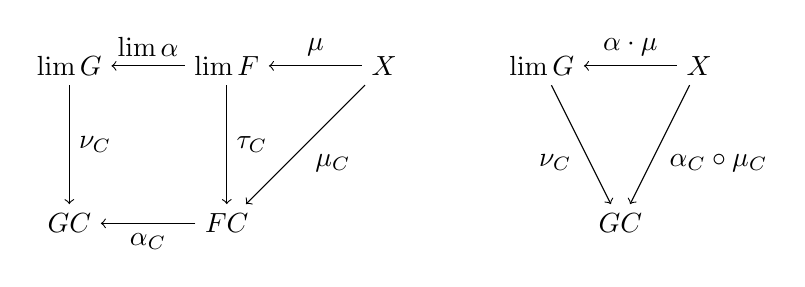
\begin{tikzpicture}[auto]
      \node (x) at (4, 0) {$X$};

      \node (limf) at (2, 0) {$\lim F$};
      \node (limg) at (0, 0) {$\lim G$};

      \node (fa) at (2, -2) {$FC$};
      \node (ga) at (0, -2) {$GC$};
      \draw[->] (x) to node{$\mu_C$}(fa);
      \draw[->] (x) to node[swap]{$\tuple{\mu}$}(limf);

      \draw[->] (limf) to node{$\tau_C$}(fa);
      \draw[->] (limg) to node{$\nu_C$}(ga);
      \draw[->] (fa) to node{$\alpha_C$}(ga);
      \draw[->] (limf) to node[swap]{$\lim \alpha$}(limg);

      \node (limf) at (6, 0) {$\lim G$};
      \node (x) at (8, 0) {$X$};

      \node (fa) at (7, -2) {$GC$};
      \draw[->] (limf) to node[swap]{$\nu_C$}(fa);
      \draw[->] (x) to node{$\alpha_C\circ\mu_C$}(fa);
      \draw[->] (x) to node[swap]{$\tuple{\alpha\cdot\mu}$}(limf);
    \end{tikzpicture}
  \end{center}
\end{proof}

\begin{prop}[共変Hom関手の極限の保存]
  \[\arset{D}{X}{\lim F}\cong\lim\arset{D}{X}{F-}\]が任意の対象$X$、任意の関手$\functor{F}{C}{D}$において自然に成り立つ。
\end{prop}
\begin{proof}[同型性]
  共変Hom関手の積の保存と同様に示す。つまり$\arset{D}{X}{\lim F}$が関手$\functor{\arset{D}{X}{F-}}{C}{Set}$の極限であることを示せば良い。
  \begin{center}
    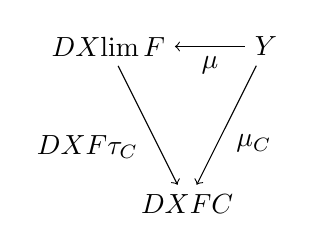
\begin{tikzpicture}[auto]
      \node (limf) at (0, 2) {$\arset{D}{X}{\lim F}$};
      \node (x) at (2, 2) {$Y$};

      \node (fa) at (1, 0) {$\arset{D}{X}{FC}$};
      \draw[->] (limf) to node[swap]{$\arset{D}{X}{F\tau_C}$}(fa);
      \draw[->] (x) to node{$\mu_C$}(fa);
      \draw[->] (x) to node{$\tuple{\mu}$}(limf);
    \end{tikzpicture}
  \end{center}
  また$\arset{D}{X}{\tau_C}$は、関手$\arset{D}{X}{-}$と自然変換$\tau$の水平合成で得られる自然変換であるため、自然性を保つ。

  Hom関手の積の保存と同様にまずは$Y$を$1$に制限する。
  \begin{center}
    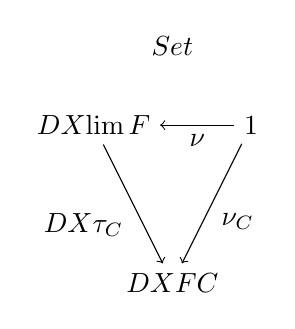
\begin{tikzpicture}[auto]
      \node (x) at (1, 3) {$\cat{Set}$};

      \node (limf) at (0, 2) {$\arset{D}{X}{\lim F}$};
      \node (x) at (2, 2) {$1$};

      \node (fa) at (1, 0) {$\arset{D}{X}{FC}$};
      \draw[->] (limf) to node[swap]{$\arset{D}{X}{\tau_C}$}(fa);
      \draw[->] (x) to node{$\nu_C$}(fa);
      \draw[->] (x) to node{$\tuple{\nu}$}(limf);
    \end{tikzpicture}
    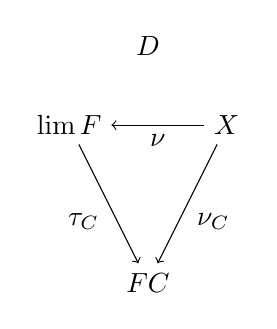
\begin{tikzpicture}[auto]
      \node (x) at (1, 3) {$\cat{D}$};

      \node (limf) at (0, 2) {$\lim F$};
      \node (x) at (2, 2) {$X$};
      \node (fa) at (1, 0) {$FC$};
      \draw[->] (limf) to node[swap]{$\tau_C$}(fa);
      \draw[->] (x) to node{$\nu_C$}(fa);
      \draw[->] (x) to node{$\tuple{\nu}$}(limf);
    \end{tikzpicture}
  \end{center}

  また圏$\cat{Set}$における$\nu$の自然性と値の適用と元の合成の同値性より、$\cat{C}$における$\nu$も自然変換となるから、$(X,\nu)$は$\cat{C}$における錐となり、一意に存在する射$\mor{\tuple{\nu}}{X}{\lim F}$が得られる。また$A\cong\arset{Set}{1}{A}$から$\arset{D}{X}{\lim F}\cong \arset{Set}{1}{\arset{D}{X}{\lim F}}$であり、$\mor{\tuple{\nu}}{1}{\arset{D}{X}{\lim F}}$もまた一意に存在し、値の適用と元の合成の同値性から図式を可換にする。
  \begin{center}
    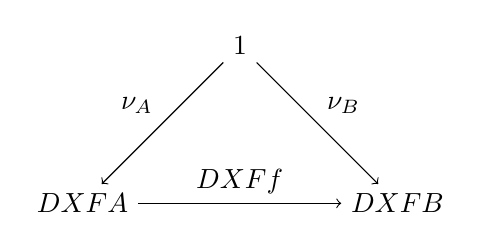
\begin{tikzpicture}[auto]
      \node (limf) at (0, 2) {$1$};
      \node (fa) at (-2, 0) {$\arset{D}{X}{FA}$};
      \node (fb) at (2, 0) {$\arset{D}{X}{FB}$};
      \draw[->] (limf) to node[swap]{$\nu_A$}(fa);
      \draw[->] (limf) to node{$\nu_B$}(fb);
      \draw[->] (fa) to node{$\arset{D}{X}{Ff}$}(fb);
    \end{tikzpicture}
  \end{center}

  一般の$Y$に戻ると、$Y$の任意の元$y$に対して極限の分配則より\[\tuple{\mu}\circ y = \tuple{\mu\cdot \varDelta y}\]であったから、任意の元$y$に対して$\mor{\tuple{\mu}\circ y}{1}{\arset{D}{X}{\lim F}}$が一意に存在する。よって射$\mor{\tuple{\mu}}{Y}{\arset{D}{X}{\lim F}}$もまた一意に存在する。
  \begin{center}
    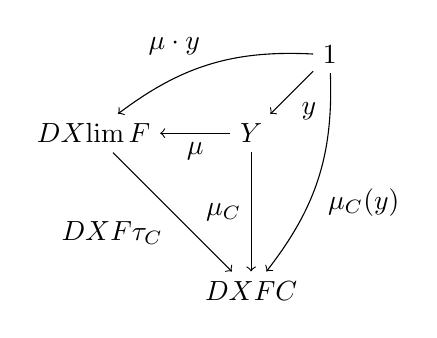
\begin{tikzpicture}[auto]
      \node (limf) at (0, 2) {$\arset{D}{X}{\lim F}$};
      \node (x) at (2, 2) {$Y$};
      \node (1) at (3, 3) {$1$};

      \node (fa) at (2, 0) {$\arset{D}{X}{FC}$};
      \draw[->] (limf) to node[swap]{$\arset{D}{X}{F\tau_C}$}(fa);
      \draw[->] (x) to node[swap]{$\mu_C$}(fa);
      \draw[->] (x) to node{$\tuple{\mu}$}(limf);
      \draw[->] (1) to node{$y$}(x);
      \draw[->,bend left = 20] (1) to node{$\mu_C(y)$}(fa);
      \draw[->,bend right = 20] (1) to node[swap]{$\tuple{\mu\cdot\varDelta y}$}(limf);
    \end{tikzpicture}
  \end{center}
  よって、$(\arset{D}{X}{\lim F},\arset{D}{X}{\tau})$は関手$\arset{D}{X}{F-}$における極限であり、極限の一意性から$\arset{D}{X}{\lim F}\cong\lim\arset{C}{X}{F-}$である。
\end{proof}
二つの極限$(\arset{D}{X}{\lim F},\arset{D}{X}{\tau})$、$(\lim \arset{D}{X}{F-},\nu)$の間の同型射は極限の一意性による証明によれば、それぞれ
\[\mor{\tuple{\arset{D}{X}{\tau}}}{\arset{D}{X}{\lim F}}{\lim \arset{D}{X}{F-}}\]
\[\mor{\tuple{\nu}}{\lim \arset{D}{X}{F-}}{\arset{D}{X}{\lim F}}\]
\begin{proof}[自然性]
  まずは$X$の自然性について考える。
  二つの極限$(\arset{D}{X}{\lim F},\arset{D}{X}{\tau})$、$(\lim \arset{D}{X}{F-},\nu)$と任意の射$\mor{f}{Y}{X}$に対して、以下の図式が可換になればよい。
  \begin{center}
    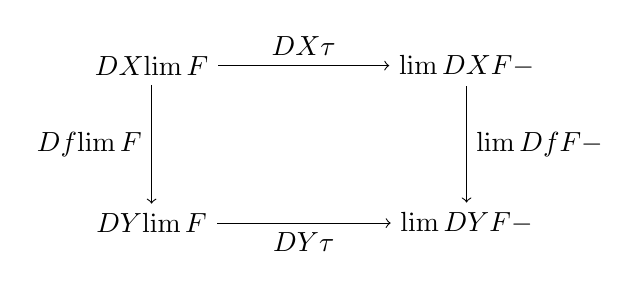
\begin{tikzpicture}[auto]
      \node (xlf) at (0, 0) {$\arset{D}{X}{\lim F}$};
      \node (ylf) at (0, -2) {$\arset{D}{Y}{\lim F}$};
      \node (lxf) at (4, 0) {$\lim\arset{D}{X}{F-}$};
      \node (lyf) at (4, -2) {$\lim\arset{D}{Y}{F-}$};

      \draw[->] (xlf) to node[swap]{$\arset{D}{f}{\lim F}$}(ylf);
      \draw[->] (lxf) to node{$\lim \arset{D}{f}{F-}$}(lyf);
      \draw[<-] (lxf) to node[swap]{$\tuple{\arset{D}{X}{\tau}}$}(xlf);
      \draw[<-] (lyf) to node{$\tuple{\arset{D}{Y}{\tau}}$}(ylf);

    \end{tikzpicture}
  \end{center}
  ここで極限の分配則より、\[\tuple{\arset{D}{Y}{\tau}}\circ\arset{D}{f}{\lim F}=\tuple{\arset{D}{Y}{\tau}\cdot\varDelta\arset{D}{f}{\lim F}}\]が成り立つ。
  また圏$\cat{C}$の任意の対象$C$に対して、
  \begin{align*}
    (\arset{D}{Y}{\tau}\cdot\varDelta \arset{D}{f}{\lim F})_C
    &=\arset{D}{Y}{\tau}_C\circ\arset{D}{f}{\lim F}&\text{(自然変換の垂直合成の定義)}\\
    &=\arset{D}{Y}{\tau_C}\circ\arset{D}{f}{\lim F}&\text{(自然変換の水平合成の定義)}\\
    &=\arset{D}{f}{\tau_C}&\text{(双Hom関手の定義)}\\
    &=\arset{D}{f}{\tau}_C&\text{(自然変換の水平合成の定義)}\\
  \end{align*}
  よって$\arset{D}{Y}{\tau}\cdot\varDelta \arset{D}{f}{\lim F}=\arset{D}{f}{\tau}$が成り立つから、
  \begin{align*}
    \tuple{\arset{D}{Y}{\tau}}\circ\arset{D}{f}{\lim F}&=\tuple{\arset{D}{Y}{\tau}}\\
  \end{align*}
  となる。もう一つの射$\lim\arset{D}{f}{F-}\circ\tuple{\arset{D}{X}{\tau}}$についても、自然変換の極限$\lim\arset{D}{f}{F-}$の適用より、
  \[\lim\arset{D}{f}{F-}\circ\tuple{\arset{D}{X}{\tau}} = \tuple{\arset{D}{f}{F-}\cdot\arset{D}{X}{\tau}}\]が成り立つ。圏$\cat{C}$の任意の対象$C$に対して、
  \begin{align*}
    (\arset{D}{f}{F-}\cdot\arset{D}{X}{\tau})_C &= \arset{D}{f}{FC}\circ\arset{D}{X}{\tau_C}&\text{(自然変換の垂直合成の定義)}\\
    &=\arset{D}{f}{\tau_C}&\text{(双Hom関手の定義)}\\
    &=\arset{D}{f}{\tau}_C&\text{(自然変換の水平合成の定義)}\\
  \end{align*}
  よって$\arset{D}{f}{F-}\cdot\arset{D}{X}{\tau}=\arset{D}{f}{\tau}$が成り立つから、\[\lim\arset{D}{f}{F-}\circ\tuple{\arset{D}{X}{\tau}}=\arset{D}{f}{\tau}\]である。
  よって\[\tuple{\arset{D}{Y}{\tau}}\circ\arset{D}{f}{\lim F}=\arset{D}{f}{\tau}=\lim\arset{D}{f}{F-}\circ\tuple{\arset{D}{X}{\tau}}\]となり、$X$に対して自然であることが分かった。

  次に$F$に対する自然性を示す。つまり任意の自然変換$\nat{\alpha}{F}{G}$と二つの極限$(\lim F,\tau)$、$(\lim G,\nu)$に対して以下の図式が可換であることを示せば良い。
  
  \begin{center}
    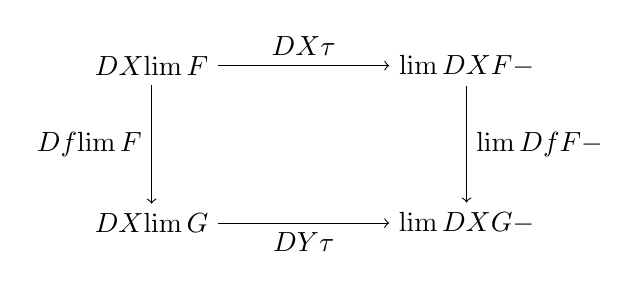
\begin{tikzpicture}[auto]
      \node (xlf) at (0, 0) {$\arset{D}{X}{\lim F}$};
      \node (ylf) at (0, -2) {$\arset{D}{X}{\lim G}$};
      \node (lxf) at (4, 0) {$\lim\arset{D}{X}{F-}$};
      \node (lyf) at (4, -2) {$\lim\arset{D}{X}{G-}$};

      \draw[->] (xlf) to node[swap]{$\arset{D}{f}{\lim F}$}(ylf);
      \draw[->] (lxf) to node{$\lim \arset{D}{f}{F-}$}(lyf);
      \draw[<-] (lxf) to node[swap]{$\tuple{\arset{D}{X}{\tau}}$}(xlf);
      \draw[<-] (lyf) to node{$\tuple{\arset{D}{Y}{\tau}}$}(ylf);
    \end{tikzpicture}
  \end{center}
  
  自然変換の極限$\lim\arset{D}{X}{\alpha}$の適用より、
  \begin{align*}
    \lim\arset{D}{X}{\alpha}\circ\tuple{\arset{D}{X}{\tau}}&=\tuple{\arset{D}{X}{\alpha}\cdot\arset{D}{X}{\tau}}&\text{(極限の分配則)}\\
    &=\tuple{\arset{D}{X}{\alpha\cdot\tau}}&\text{(相互交換法則)}\\
  \end{align*}
  同様に極限の分配則より、
  \begin{align*}
    \tuple{\arset{D}{X}{\nu}}\circ\arset{D}{X}{\lim \alpha}
    &=\tuple{\arset{D}{X}{\nu}}\circ\arset{D}{X}{\lim \tuple{\alpha\cdot\tau}}&\text{(極限関手の射関数の定義)}\\
    &=\tuple{\arset{D}{X}{\nu}\cdot\varDelta \arset{D}{X}{\tuple{\alpha\cdot\tau}}}&\text{(極限の分配則)}\\
  \end{align*}
  が成り立つ。ここで圏$\cat{C}$の任意の対象$C$において、
  \begin{align*}
    (\arset{D}{X}{\nu}\cdot\varDelta \arset{D}{X}{\tuple{\alpha\cdot\tau}})_C
    &=\arset{D}{X}{\nu_C}\circ\arset{D}{X}{\tuple{\alpha\cdot\tau}}&\text{(自然変換の垂直合成の定義)}\\
    &=\arset{D}{X}{\nu_C\circ\tuple{\alpha\cdot\tau}}&\text{(Hom関手の合成の保存)}\\
    &=\arset{D}{X}{(\alpha\cdot\tau)_C}&\text{(射影射$\nu$による分解)}\\
    &=\arset{D}{X}{(\alpha\cdot\tau)}_C
  \end{align*}
  となるから$\arset{D}{X}{\nu}\cdot\varDelta \arset{D}{X}{\tuple{\alpha\cdot\tau}}=\arset{D}{X}{(\alpha\cdot\tau)}$となって、
  \[\tuple{\arset{D}{X}{\nu}}\circ\arset{D}{X}{\lim \alpha}=\arset{D}{X}{(\alpha\cdot\tau)}\]が成り立ち、

  \[\lim\arset{D}{X}{\alpha}\circ\tuple{\arset{D}{X}{\tau}}=\arset{D}{X}{(\alpha\cdot\tau)}=\tuple{\arset{D}{X}{\nu}}\circ\arset{D}{X}{\lim \alpha}\]となるから$F$に対して自然である。
\end{proof}
